% =====================================================================
%  MathFest 2026 Poster -- 36 in x 36 in
%  "What Can a Persistence Diagram See?"
%  Christian Dane Beels, advised by Dr. Joseph Dorta
%  Template base: Sofia Jijon (https://sjijon.github.io)
%
%  LAYOUT: three independent, equal-width columns.
%    - Left: motivation, TDA background and related work, then the proof.
%    - Middle: research question and the empirical results.
%    - Right: experimental design, discussion/conclusion, and references.
%
%  SPACING: all column separation is controlled by colspace. There are no
%  subcolumns in this version.
% =====================================================================

\documentclass[a0paper,portrait,margin=0mm,colspace=52pt,blockverticalspace=40pt,innermargin=0pt]{tikzposter}
\geometry{paperwidth=36in,paperheight=36in,margin=0mm}

\usepackage[latin9]{inputenc}
\usepackage{amsmath,amssymb}
\usepackage{enumitem}
\usepackage{multicol}
% \usepackage[colalign]{aligncolsatbottom}
% ^ DISABLED (Phase V6): aligncolsatbottom is not on CTAN and is not in the
% MiKTeX package database, so this line is a hard build failure, not the
% "untested interaction" the original header anticipated. Its only effect was
% cosmetic bottom-alignment of columns. Restore only if you obtain the .sty.

\setlist[itemize]{leftmargin=*,itemsep=2pt,topsep=1pt,parsep=0pt,partopsep=0pt}

% Body font for block text. tikzposter's a0 \normalsize is 24.88pt/30pt, which
% overflowed the bottom margin in the right column (measured: content reached
% 35.60 in against a 35.20 in limit). 22.8pt/27.4pt was found by compiling and
% measuring: it fills the page and leaves References and Contact bottoms within
% 0.15 in of each other. Change in ONE place to trade text against figure size.
\newcommand{\bodyfont}{\fontsize{22.8}{27.4}\selectfont}

%......................................................................
\tikzposterlatexaffectionproofoff
\usetikzlibrary{shapes.geometric,arrows.meta,positioning}

\usepackage{helvet}
\renewcommand{\familydefault}{\sfdefault}

\definecolor{MyFadedNavy}{rgb}{0.224, 0.259, 0.310}
\definecolor{MyTerracotta}{rgb}{0.914, 0.310, 0.216}
\definecolor{MyIvory}{rgb}{0.965, 0.969, 0.922}

\usetheme{Default}
\definecolorstyle{MyStyle2016}{
	\definecolor{ColorOne}{named}{MyFadedNavy}
	\definecolor{ColorTwo}{named}{MyTerracotta}
	\definecolor{ColorThree}{named}{MyIvory}
}{
    \colorlet{titlebgcolor}{ColorOne}
    \colorlet{titlefgcolor}{white}
    \colorlet{backgroundcolor}{ColorOne!15}
    \colorlet{framecolor}{ColorOne}
    \colorlet{blocktitlebgcolor}{white}
    \colorlet{blocktitlefgcolor}{ColorTwo}
    \colorlet{blockbodybgcolor}{white}
    \colorlet{blockbodyfgcolor}{black}
    \colorlet{innerblocktitlebgcolor}{ColorOne!15}
    \colorlet{innerblocktitlefgcolor}{black}
    \colorlet{innerblockbodybgcolor}{ColorOne!15}
    \colorlet{innerblockbodyfgcolor}{black}
    \colorlet{notebgcolor}{ColorTwo!20}
    \colorlet{notefgcolor}{ColorTwo}
    \colorlet{notefrcolor}{ColorTwo}
 }

\usecolorstyle{MyStyle2016}
%......................................................................
\title{\parbox{0.92\linewidth}{\centering What Can a Persistence Diagram See?\\[0.3cm]
{\Large Invariance Structure and the Detectability of Data Poisoning}}}

\author{\underline{Christian Dane Beels}, Dr.\ Joseph Dorta}

\institute{Department of Mathematical Sciences\\United States Military Academy, West Point, NY.}

%......................................................................
\begin{document}

\maketitle[width=0.96\linewidth,titletoblockverticalspace=24pt,linewidth=0,roundedcorners=10]

\begin{columns}
%======================================================================
%  LEFT COLUMN -- motivation, background, and proof
%======================================================================
\column{0.333}

\block[titleleft,roundedcorners=16]{Motivation}{
	\bodyfont\raggedright
	\begin{itemize}
		\item Modern Network Intrusion Detection Systems (NIDS) rely on ML models vulnerable to \textbf{data poisoning}: a cyber attack in which adversaries inject biased data to degrade model accuracy / performance.
		\item Defenses must run \textbf{before training}, so clustering is unsupervised --- there are no labels to use.\\
        \begin{center}
            
\includegraphics[width=\linewidth]{Figures/figure_v5_nids_poisoning}
        \end{center}
	\end{itemize}
}

\block[titleleft,roundedcorners=16]{TDA Background and Related Work}{
	\bodyfont\raggedright
	\begin{itemize}
        \item TDA uses concepts from topology to study the global "shape" of data (connections and clusters between data points)
        \item Persistent homology tracks topological features (connected components = $H_0$, loops = $H_1$) as a radius parameter is increased - features that persist over longer ranges are more significant
		\item \textbf{Related work:} Monkam et al.\ [1] use TDA as a pre-training filter for poisoned NIDS data, motivating the question of which perturbations their TDA lens can see.
	\end{itemize}
    \begin{center}
  
\includegraphics[width=\linewidth]{Figures/figure_v1_tda_background}
\end{center}
}

\block[titleleft,roundedcorners=16]{The Argument}{
	\bodyfont\raggedright

	A reordering attack applies a permutation $\large\sigma\in S_{1500}$ to the positions of a packet's 1,500 payload bytes. It changes \emph{where} byte values appear, but not the collection of byte values itself:
	\begin{equation}
    \Large
		x \xrightarrow{\ \sigma\in S_{1500}\ } x\circ\sigma .
		\tag{1}
	\end{equation}

	Binarization acts independently at each byte position. Therefore, reordering before binarization gives the same result as binarizing first and then reordering:
	\begin{equation}
    \Large
		b(x\circ\sigma)=b(x)\circ\sigma .
		\tag{2}
	\end{equation}

	The binarized image is thus \textbf{equivariant}: it moves when the packet is reordered. However, the foreground-count feature sums over all positions. Because $\sigma$ is a bijection, it only rearranges the summands:
	\begin{equation}
    \Large
		\sum_{i=1}^{1500} b\!\left((x\circ\sigma)_i\right)
		=
		\sum_{i=1}^{1500} b(x_{\sigma(i)})
		=
		\sum_{i=1}^{1500} b(x_i).
		\tag{3}
	\end{equation}

	Thus, the foreground count is \textbf{invariant} under every permutation, not merely the attacks tested here. The threshold is fitted using a batch maximum; maxima are also permutation-invariant, and this was verified in code. Count-derived features are therefore provably insensitive to byte-position reordering.

	\begin{center}
	
\includegraphics[width=\linewidth]{Figures/figure_v2_binarized_triptych}
	\end{center}

	\innerblock{}{\centering\textbf{Residual capture must come from outside the count channel.}}
}

%======================================================================
%  MIDDLE COLUMN -- research question and results
%======================================================================
\column{0.333}

\block[titleleft,roundedcorners=16]{Research Question}{
	\raggedright
	\innerblock{}{
		\centering
		\textbf{What determines a data poisoning attack's topological detectability --- and can a more sophisticated attack lead to less detectable topological signatures?}
	}
}

\block[titleleft,roundedcorners=16]{Main Result: Detectability Tracks Spatial Disruption}{
    \bodyfont\centering

    \innerblock{}{
    \centering
    \textbf{What did we investigate?}\\
    Which poisoned-packet perturbations can a TDA-based NIDS filter detect?\\[0.35cm]

    \textbf{Main result}\\
    \textbf{Detectability tracks spatial disruption, not attack sophistication.}\\[0.35cm]

    \textbf{Evidence}\\
    All four reordering attacks preserve foreground counts ($0/1{,}600$ changes),
    yet capture rises from $0\%$ for localized operations to $6.28\%$ for cyclic
    shift. Surrogate-guided search reaches a comparable $6.48\%$.
    }

    \begin{center}
        
\includegraphics[width=\linewidth]{Figures/figure_v3_four_families}
    \end{center}

    \small\raggedright
    \textbf{How to read Figure V3.} Each attack preserves the same payload-byte
    multiset and therefore leaves the foreground-count channel unchanged. What
    differs is the amount of meaningful spatial rearrangement. Localized block
    operations produce no capture, while the full cyclic shift produces the
    largest capture among the four reordering families.

    \begin{center}
        
\includegraphics[width=0.88\linewidth]{Figures/figure_v4_guidance_shift}
    \end{center}

    \small\raggedright
    \textbf{Companion evidence.} Guidance improves capture over random swaps,
    but does not outperform a trivial cyclic shift. The important variable is
    spatial disruption, not whether the attack is sophisticated.
}

%======================================================================
%  RIGHT COLUMN -- design, interpretation, and references
%======================================================================
\column{0.333}

\block[titleleft,roundedcorners=16]{Experimental Design}{
	\centering
	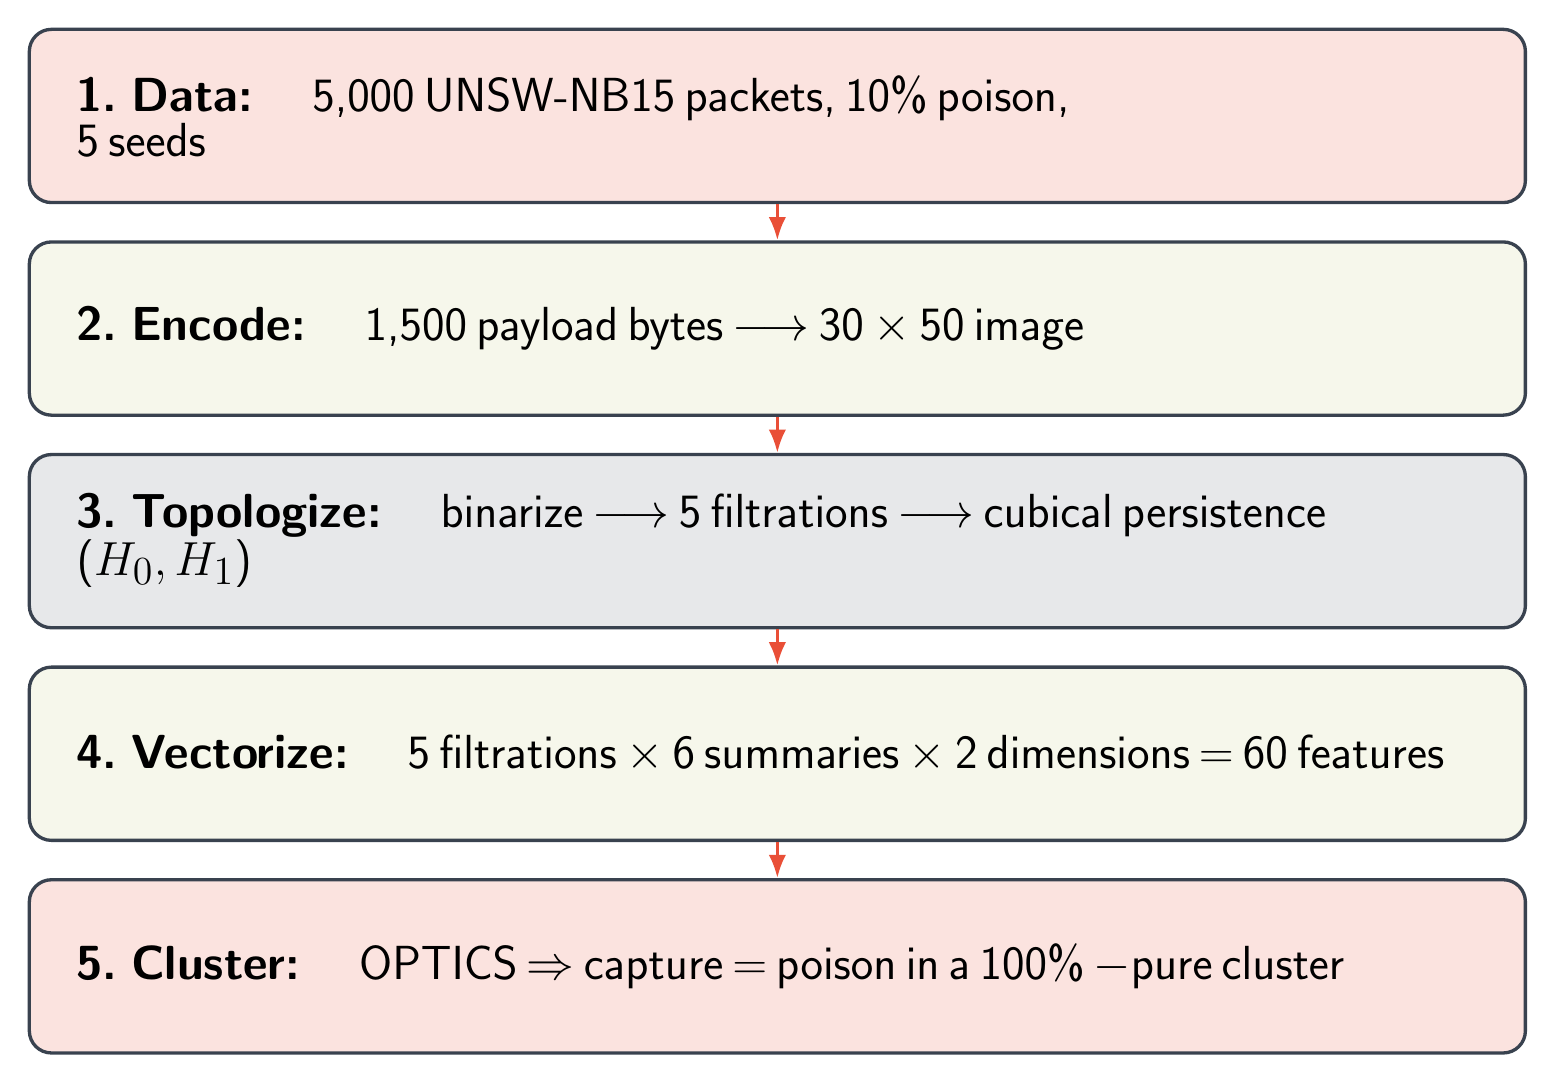
\begin{tikzpicture}[>=Latex,
		card/.style={draw=MyFadedNavy, line width=1.2pt, rounded corners=8pt,
			align=left, minimum width=19cm, minimum height=2.2cm,
			text width=17.8cm, inner sep=4pt},
		arrow/.style={->, very thick, MyTerracotta}]
		\node[card, fill=MyTerracotta!16] (data) at (0,0)
			{\fontsize{19}{22}\selectfont\textbf{1. Data:} \quad 5,000 UNSW-NB15 packets, 10\% poison, \\ 5 seeds};
		\node[card, fill=MyIvory] (image) at (0,-2.70)
			{\fontsize{19}{22}\selectfont\textbf{2. Encode:} \quad 1,500 payload bytes $\longrightarrow$ 30 $\times$ 50 image};
		\node[card, fill=MyFadedNavy!12] (tda) at (0,-5.40)
			{\fontsize{19}{22}\selectfont\textbf{3. Topologize:} \quad binarize $\longrightarrow$ 5 filtrations $\longrightarrow$ cubical persistence ($H_0,H_1$)};
		\node[card, fill=MyIvory] (features) at (0,-8.10)
			{\fontsize{19}{22}\selectfont\textbf{4. Vectorize:} \quad 5 filtrations $\times$ 6 summaries $\times$ 2 dimensions $=$ 60 features};
		\node[card, fill=MyTerracotta!16] (cluster) at (0,-10.80)
			{\fontsize{19}{22}\selectfont\textbf{5. Cluster:} \quad OPTICS $\Rightarrow$ capture $=$ poison in a 100\% $-$pure cluster};
		\draw[arrow] (data.south) -- (image.north);
		\draw[arrow] (image.south) -- (tda.north);
		\draw[arrow] (tda.south) -- (features.north);
		\draw[arrow] (features.south) -- (cluster.north);
	\end{tikzpicture}

	\raggedright\small
	Four multiset-preserving reordering families; Gaussian noise is the positive control. Reported $\pm$ values are population SD across five seeds.
}

\block[titleleft,roundedcorners=16]{Discussion and Conclusion}{
	\bodyfont\raggedright
	\begin{itemize}
		\item \textbf{A feature-map blind spot can be read from the algebra before experimentation.}
		\item \textbf{Insensitive is not undetectable:} detectability belongs to the \emph{attack--detector pair}, not to permutation invariance alone.
		\item Guidance increases capture over random swaps, yet does not outperform a trivial shift: \textbf{spatial disruption matters more than sophistication.}
		\item \textbf{Next:} isolate the residual signal by filtration. Guidance does not replicate on CICIDS2017 ($-0.60\pm3.03$).
	\end{itemize}

	\innerblock{}{
		\small
		\textbf{Scope.} Proof: any fixed-threshold pipeline. Empirics: one reconstruction, five seeds, one primary dataset; cross-dataset guidance did not replicate.
	}
}


\block[titleleft,roundedcorners=16]{References}{
\fontsize{16}{19}\selectfont
\begin{itemize}[itemsep=2pt,leftmargin=*]
	\item[{[1]}] G. F. Monkam, M. J. De Lucia, and N. D. Bastian, ``A topological data analysis approach for detecting data poisoning attacks against machine learning based network intrusion detection systems,'' \emph{Computers \& Security}, vol.\ 144, art.\ no.\ 103929, Sep.\ 2024.
	\item[{[2]}] M. Ferrara, ``Modeling by topological data analysis and game theory for analyzing data poisoning phenomena,'' \emph{AIMS Mathematics}, vol.\ 10, no.\ 7, pp.\ 15457--15475, Jul.\ 2025.
	\item[{[3]}] D. Cohen-Steiner, H. Edelsbrunner, and J. Harer, ``Stability of persistence diagrams,'' in \emph{Proc.\ 21st Annu.\ Symp.\ Computational Geometry (SCG '05)}, Pisa, Italy, Jun.\ 2005, pp.\ 263--271.
	\item[{[4]}] M. G. Bergomi, P. Frosini, D. Giorgi, and N. Quercioli, ``Towards a topological--geometrical theory of group equivariant non-expansive operators for data analysis and machine learning,'' \emph{Nature Machine Intelligence}, vol.\ 1, pp.\ 423--433, 2019.
	\item[{[5]}] A. Garin and G. Tauzin, ``A topological reading lesson: Classification of MNIST using TDA,'' arXiv:1910.08345, 2019.
\end{itemize}
}

% Contact moved here (was bottom of the left subcolumn) so that it sits at
% bottom-right, opposite the References strip at bottom-left.

\iffalse
\block[titleleft,roundedcorners=16]{Contact}{
	\small
	\raggedright
	\textbf{Christian Dane Beels} \quad christian.beels@westpoint.edu\\
	github.com/cdaneb/ \quad linkedin.com/in/christiandanebeels/\\
	Dept.\ of Mathematical Sciences, USMA West Point
}
\fi

\end{columns}
\end{document}
